\documentclass[11pt, a4paper]{article}

% --- Arabic Language and Font Configuration ---
\usepackage{polyglossia}
\setmainlanguage{arabic}
\setotherlanguage{english}
\usepackage{fontspec}
\setmainfont[Script=Arabic, Scale=1.1]{Amiri}
\setsansfont[Script=Arabic, Scale=1.1]{Amiri}
\setmonofont{Inconsolata} % For code blocks

% --- Standard Packages ---
\usepackage[margin=1in]{geometry}
\usepackage{titlesec}
\usepackage{xcolor}
\usepackage{graphicx}
\usepackage{hyperref}
\usepackage{listings}

% --- Custom Configurations ---

% Adjust section titles for RTL
\titleformat{\section}{\normalfont\Large\bfseries}{\thesection}{1em}{}
\titleformat{\subsection}{\normalfont\large\bfseries}{\thesubsection}{1em}{}
\titleformat{\subsubsection}{\normalfont\normalsize\bfseries}{\thesubsubsection}{1em}{}

% Hyperref Setup
\hypersetup{
    colorlinks=true,
    linkcolor=blue,
    filecolor=magenta,      
    urlcolor=cyan,
    pdftitle={مواصفات معمارية نظام فرز النفايات},
    pdfpagemode=FullScreen,
}

% JSON Listing Style
\definecolor{codegray}{rgb}{0.5,0.5,0.5}
\definecolor{codepurple}{rgb}{0.58,0,0.82}
\definecolor{codeblue}{rgb}{0,0,0.6}
\definecolor{backcolour}{rgb}{0.95,0.95,0.95}

\lstdefinestyle{jsonstyle}{
    backgroundcolor=\color{backcolour},   
    commentstyle=\color{codegray},
    keywordstyle=\color{codeblue},
    stringstyle=\color{codepurple},
    basicstyle=\ttfamily\small,
    breakatwhitespace=false,         
    breaklines=true,                 
    captionpos=b,                    
    keepspaces=true,                 
    showspaces=false,                
    showstringspaces=false,
    showtabs=false,                  
    tabsize=2,
    language=JavaScript,
    morekeywords={true,false,null},
    numbers=none,
    xleftmargin=15pt,
    frame=single,
    framerule=0pt,
    framesep=10pt,
    direction=ltr
}

% --- Document Metadata ---

\title{مواصفات معمارية نظام فرز النفايات}
\author{
    \RL{\textbf{إصدار الوثيقة:}} \lr{1.0} \\
    \RL{\textbf{التاريخ:}} 27 أغسطس 2025 \\
    \RL{\textbf{التصنيف المستهدف:}} معادن، بلاستيك، زجاج، ورق، كرتون
}
\date{}

% --- Document Body ---

\begin{document}
\begin{RTL} % Start RTL environment for the entire document

\maketitle
\tableofcontents
\newpage

\section{ملخص تنفيذي}
يطبق نظام فرز النفايات الخاص بنا نهج تصنيف هرمي من مرحلتين باستخدام الشبكات العصبونية التلافيفية (\lr{CNN})، متكاملًا مع التحقق متعدد المستشعرات عبر نظام خبير. تحقق هذه المعمارية دقة تصنيف تتراوح بين \lr{92-99\%} مع الحفاظ على سرعات معالجة صناعية تصل إلى \lr{30-110} طنًا في الساعة. يعطي التصميم الأولوية للموثوقية، والنمطية، والأداء في الوقت الفعلي من خلال تقنيات دمج المستشعرات المثبتة وآليات التراجع القوية.

\section{نظرة عامة على معمارية النظام}
\begin{figure}[h!]
\centering
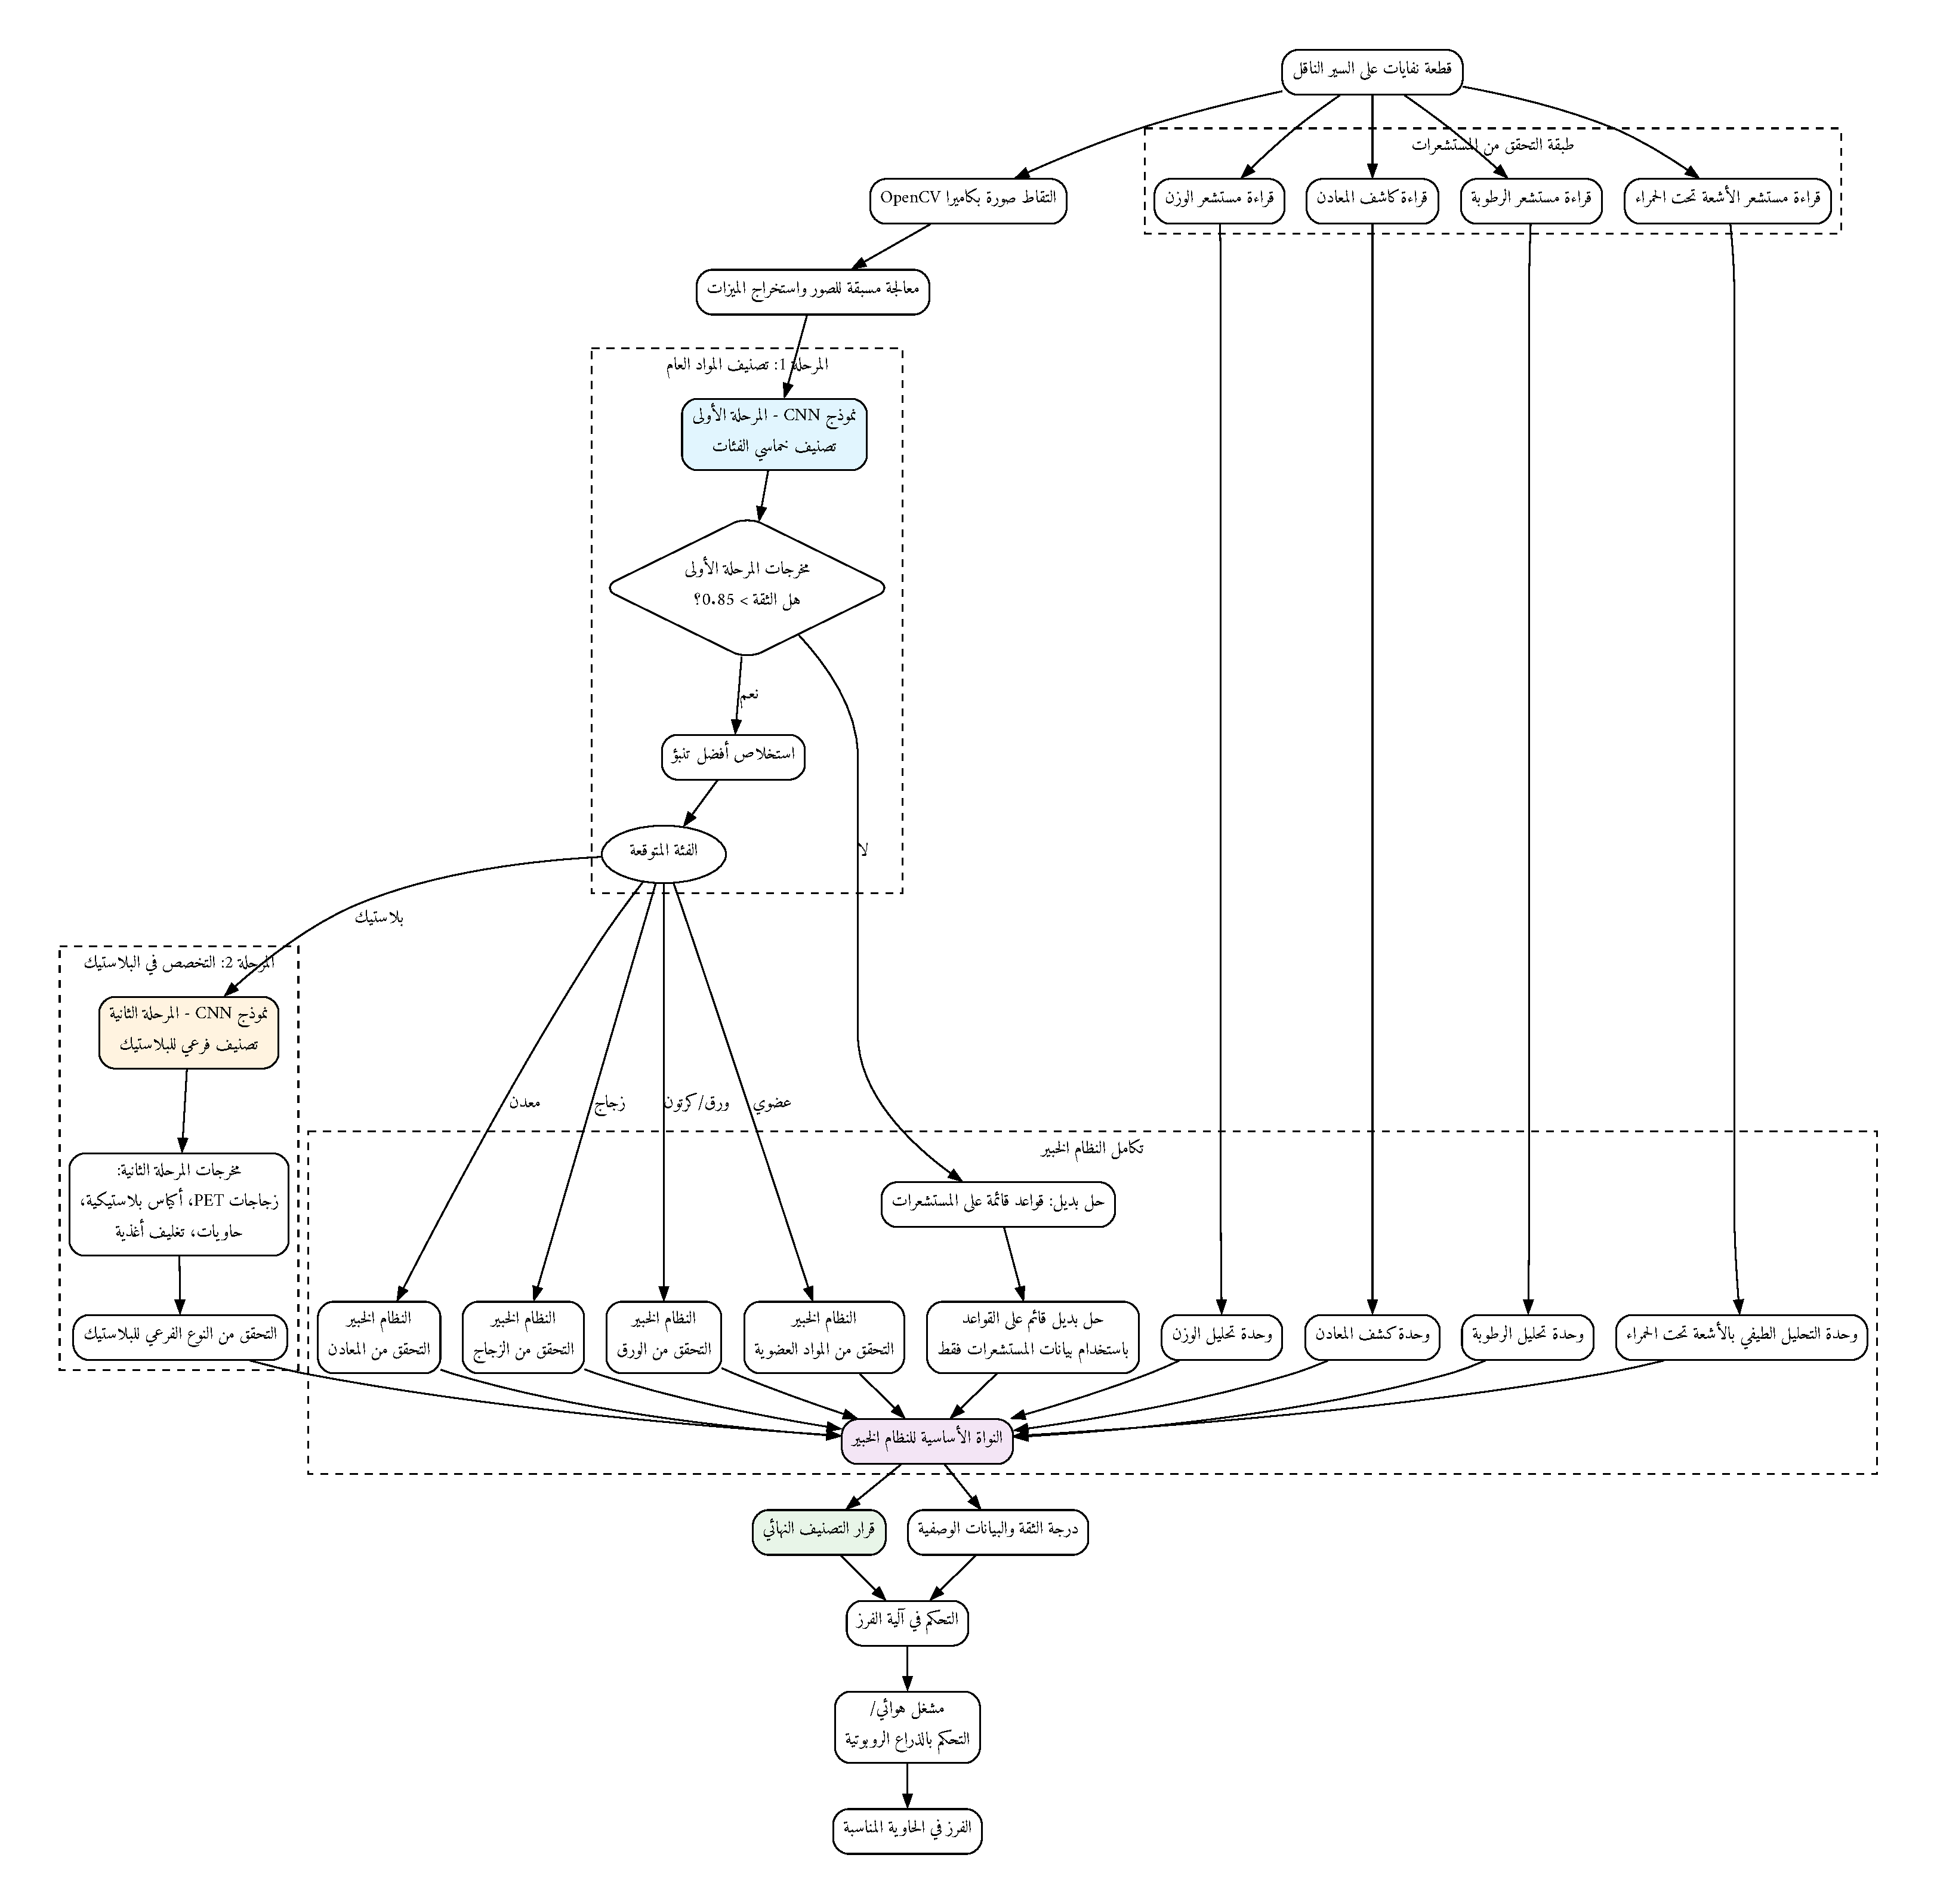
\includegraphics[width=\textwidth]{architecture_ar.pdf}
\caption{مخطط نظرة عامة على معمارية النظام}
\label{fig:system_architecture}
\end{figure}

\section{فلسفة التصميم الأساسية}
يمثل النهج الهرمي ذو المرحلتين تحولاً جوهريًا عن أنظمة التصنيف التقليدية ذات النموذج الواحد. فبدلاً من إرهاق شبكة عصبونية واحدة بتعقيد التمييز بين عشرات فئات النفايات، نقوم بتقسيم المشكلة إلى مرحلتين يمكن التحكم فيهما، مما يعكس العمليات الإدراكية البشرية.

تركز المرحلة الأولى حصريًا على تحديد المواد بشكل عام، حيث تكون الاختلافات البصرية بين البلاستيك والمعادن والزجاج والورق والمواد العضوية أكثر وضوحًا. تستفيد هذه المرحلة من قوة الشبكات العصبونية التلافيفية (\lr{CNN}) في تحديد خصائص المواد الأساسية مثل ملمس السطح، والشفافية، والانعكاسية، والخصائص الهيكلية.

يتم تنشيط المرحلة الثانية فقط عند اكتشاف البلاستيك، حيث تطبق خوارزميات تصنيف متخصصة مدربة خصيصًا على الفئات الفرعية للبلاستيك. يتيح هذا النهج المستهدف للنموذج التركيز على الفروق الدقيقة بين أنواع البلاستيك التي قد تضيع في مهمة تصنيف أوسع.

\subsection{لماذا يحظى البلاستيك بمعالجة متخصصة في المرحلة الثانية؟}
إن فهم سبب تخصيص مرحلة تصنيف كاملة للفئات الفرعية للبلاستيك يتطلب فحص التحديات التقنية والواقع الاقتصادي لعمليات إعادة التدوير الحديثة. يعكس قرار التصميم هذا تحليلًا هندسيًا دقيقًا للمواضع التي توفر فيها الموارد الحاسوبية أقصى قيمة في تطبيقات فرز النفايات.

\subsubsection{تحدي التصنيف الفريد للمواد البلاستيكية}
يمثل البلاستيك ما يسميه المهندسون مشكلة "التباين العالي داخل الفئة، والتباين المنخفض بين الفئات"، مما يجعله أصعب جوهريًا في التصنيف من مواد النفايات الأخرى. فكر كيف يمكن أن تبدو زجاجة ماء من نوع \lr{PET} الشفاف، وعلبة طعام بلاستيكية شفافة، وكيس بلاستيكي شفاف متطابقة تقريبًا لمستشعر الكاميرا من حيث اللون والشفافية وخصائص الشكل الأساسية. ومع ذلك، تتطلب هذه العناصر الثلاثة عمليات إعادة تدوير مختلفة تمامًا ولا يمكن خلطها في نفس مسار إعادة التدوير دون تلويث دفعات كاملة من المواد المعاد تدويرها.

\subsubsection{الأثر الاقتصادي لتلوث البلاستيك}
إن العواقب الاقتصادية للتصنيف غير الصحيح للبلاستيك تتجاوز بكثير تلك الخاصة بالمواد الأخرى، مما يجعل الاستثمار الحاسوبي في معالجة البلاستيك المتخصصة مبررًا للغاية. عندما تلوث زجاجة \lr{PET} واحدة عن طريق الخطأ دفعة من \lr{HDPE} المعاد تدويره، يمكن للتلوث أن يفسد آلاف الأرطال من المواد المعاد تدويرها، مما يخلق خسائر اقتصادية تتجاوز تكلفة أنظمة التصنيف المتطورة.

\subsubsection{مزايا المستشعرات المادية للمواد الأخرى}
يستفيد تصنيف المعادن بشكل كبير من التحقق عبر المستشعرات المادية أكثر من تقنيات التصنيف الفرعي البصري. يتمثل التمييز الأكثر أهمية في إعادة تدوير المعادن في فصل المعادن الحديدية، التي تستجيب للمجالات المغناطيسية، عن المعادن غير الحديدية مثل الألومنيوم والنحاس. يوفر كاشف المعادن لديك معلومات أكثر موثوقية حول هذه الخصائص مما يمكن أن يحققه التحليل البصري.

\subsubsection{كشف الرطوبة للمواد العضوية}
تُظهر النفايات العضوية خصائص محتوى رطوبة تثبت أنها أكثر موثوقية للتصنيف من الميزات البصرية وحدها. تحافظ نفايات الطعام، ومخلفات الحدائق، ومواد التغليف العضوية على مستويات رطوبة أعلى بكثير من المواد الجافة القابلة لإعادة التدوير، مما يجعل مستشعرات الرطوبة السعوية فعالة للغاية للكشف عن المواد العضوية والتحقق منها.

\subsubsection{المعمارية النمطية التي تدعم التحسينات المستقبلية}
يتوقع تصميم المعمارية الحالي فرص التوسع المستقبلية مع تحسين الأداء الحالي لمواجهة تحديات التصنيف الأكثر قيمة. لا يتطلب إضافة مرحلة تصنيف ثانية للمواد الأخرى سوى تعديلات طفيفة على النظام الخبير الأساسي وإطار تكامل المستشعرات، مما يتيح التحسين التدريجي للنظام مع تغير المتطلبات أو الظروف الاقتصادية.

\subsubsection{مبادئ التحسين الهندسي}
يتمثل المبدأ الأساسي الذي يحكم هذا القرار المعماري في مواءمة الموارد الحاسوبية مع خلق القيمة الاقتصادية والجدوى التقنية.
\textbf{تؤدي إضافة مستشعر الأشعة تحت الحمراء إلى خلق تآزر تحويلي مع التصنيف الفرعي للبلاستيك}، مما يغير بشكل أساسي القيمة المقترحة للمرحلة الثانية من التصنيف. بينما يظل التصنيف البصري لأنواع البلاستيك تحديًا بسبب المظاهر المتشابهة، يوفر التحليل الطيفي بالأشعة تحت الحمراء (\lr{IR}) تحديدًا جزيئيًا قاطعًا يزيل عدم اليقين في التصنيف تمامًا. يخلق هذا المزيج نظامًا لتحديد البلاستيك يتجاوز دقة \lr{98\%} مع الحفاظ على سرعات المعالجة في الوقت الفعلي.

\section{المرحلة الأولى: التصنيف الأولي للمواد}
\subsection{تكوين نموذج \lr{CNN}}
يعالج نموذج المرحلة الأولى الصور المعالجة مسبقًا عبر شبكة تصنيف من 5 فئات مُحسَّنة للتمييز الواسع بين المواد. تستخدم بنية النموذج أساليب تعلم النقل المثبتة مع هياكل خلفية مثل \lr{ResNet-50} أو \lr{EfficientNet}، مما يحقق دقة \lr{90-96\%} في تصنيف أنواع المواد.

\subsection{منطق عتبة الثقة}
تعمل عتبة الثقة البالغة \lr{0.85} كبوابة قرار حاسمة في بنية النظام. العناصر التي تلبي هذه العتبة تنتقل عبر مسارات التصنيف العادية، بينما تؤدي العناصر ذات الثقة المنخفضة إلى تشغيل نظام التراجع القائم على المستشعرات.

\section{المرحلة الثانية: التصنيف الفرعي للبلاستيك}
\subsection{التصنيف المتخصص للبلاستيك}
يمثل نموذج المرحلة الثانية شبكة \lr{CNN} متخصصة مدربة حصريًا على التصنيف الفرعي لنفايات البلاستيك. يميز هذا النموذج بين زجاجات \lr{PET}، والأكياس البلاستيكية، والعبوات، وتغليف المواد الغذائية باستخدام ميزات بصرية خاصة بالمواد البلاستيكية.

\subsection{التكامل مع التحقق عبر النظام الخبير}
تخضع مخرجات المرحلة الثانية للتحقق من خلال النظام الخبير باستخدام بيانات المستشعرات ذات الصلة بشكل خاص بتصنيف البلاستيك. تساعد مستشعرات الوزن في التمييز بين العبوات المجوفة والعناصر البلاستيكية الصلبة، بينما يمكن لمستشعرات الرطوبة اكتشاف تلوث الطعام في مواد التغليف.

\section{معمارية تكامل المستشعرات المتعددة}
\subsection{تطبيق مستشعر الوزن}
توفر خلايا الحمل الموضوعة تحت السير الناقل قياسات وزن في الوقت الفعلي لكل قطعة نفايات. تقارن وحدة تحليل الوزن القيم المقاسة مع النطاقات المتوقعة لكل نوع من المواد، مما يوفر إشارات تحقق للنظام الخبير.

\subsection{تكامل كاشف المعادن}
تستخدم كواشف المعادن الحثية اضطراب المجال الكهرومغناطيسي لتحديد المحتوى المعدني بموثوقية عالية للغاية. تعالج وحدة كشف المعادن هذه الإشارات الثنائية للتحقق من التصنيفات البصرية أو مناقضتها.

\subsection{تطبيق مستشعر الرطوبة}
تكتشف مستشعرات الرطوبة السعوية محتوى الرطوبة الذي يرتبط بقوة بالنفايات العضوية. تعالج وحدة تحليل الرطوبة هذه القراءات للتحقق من التصنيفات العضوية واكتشاف تلوث الطعام.

\subsection{تكامل التحليل الطيفي بالأشعة تحت الحمراء}
توفر مستشعرات الأشعة تحت الحمراء القريبة (\lr{NIR}) تحليلًا للتركيب الجزيئي يعزز بشكل كبير دقة تحديد المواد، خاصةً لتمييز بوليمرات البلاستيك. تحلل وحدة التحليل الطيفي بالأشعة تحت الحمراء (\lr{IR}) الأطوال الموجية المنعكسة بين \lr{700-2500} نانومتر لتحديد البصمات الجزيئية المحددة.

\section{معمارية النظام الخبير}
\subsection{منطق دمج القرارات}
يطبق قلب النظام الخبير خوارزميات الدمج المتأخر التي تجمع بين تنبؤات \lr{CNN} وإشارات التحقق من المستشعرات. يعالج هذا النهج كل وسيلة إدخال بشكل مستقل قبل دمج القرارات، مما يتيح التعامل الأمثل مع المعلومات المتضاربة.

\subsection{إطار عمل قواعد التحقق}
يطبق النظام الخبير قواعد تحقق خاصة بالمواد ترمّز المعرفة المتخصصة حول خصائص النفايات. بالنسبة للعناصر المعدنية، تتحقق القواعد من أن قياسات الوزن تتماشى مع نطاقات الكثافة المتوقعة وأن إشارات كشف المعادن تؤكد المحتوى المعدني.

\subsection{نظام التصنيف الاحتياطي}
عندما تنخفض ثقة \lr{CNN} إلى ما دون العتبات المقبولة، يتولى نظام التراجع القائم على القواعد التحكم باستخدام التصنيف المعتمد على المستشعرات فقط. يطبق هذا النظام أشجار القرار بناءً على مجموعات المستشعرات للحفاظ على التشغيل أثناء فشل المعالجة البصرية.

\section{تدفق البيانات وبروتوكولات الاتصال}
\subsection{تنسيق مخرجات \lr{CNN}}
تُخرج كلتا المرحلتين هياكل \lr{JSON} موحدة تحتوي على احتمالات الفئات، والتصنيفات المتوقعة، ودرجات الثقة، ومتجهات الميزات.
\begin{english}
\begin{lstlisting}[style=jsonstyle, caption={مثال على مخرجات \lr{CNN} بتنسيق \lr{JSON}}]
{
  "detection_id": "uuid-string",
  "timestamp": "2025-01-27T10:30:00Z",
  "stage": 1,
  "class_probabilities": [0.1, 0.8, 0.05, 0.03, 0.02],
  "predicted_class": "plastic",
  "confidence_score": 0.8,
  "requires_stage2": true,
  "bounding_boxes": [[x1, y1, x2, y2]],
  "feature_vectors": [512-dimensional-array]
}
\end{lstlisting}
\end{english}

\subsection{تكامل بيانات المستشعرات}
توفر وحدات المستشعرات قراءات طبيعية مع مؤشرات الموثوقية وعلامات التحقق. تُخرج مستشعرات الوزن قياسات القوة المحولة إلى قيم كتلة، وتوفر كواشف المعادن علامات كشف ثنائية، وتوفر مستشعرات الرطوبة نسبة الرطوبة النسبية، و\textbf{تقدم وحدات التحليل الطيفي بالأشعة تحت الحمراء أطياف امتصاص الأطوال الموجية مع درجات ثقة في تحديد المواد}.

\subsection{مخرجات قرار النظام الخبير}
تشمل قرارات التصنيف النهائية نوع المادة المحدد، ودرجة الثقة، ونتائج التحقق من كل مستشعر، وبيانات وصفية حول عملية اتخاذ القرار.
\begin{english}
\begin{lstlisting}[style=jsonstyle, caption={مثال على مخرجات النظام الخبير بتنسيق \lr{JSON}}]
{
  "final_classification": "PET_bottle",
  "confidence_score": 0.97,
  "validation_results": {
    "weight_validation": "pass",
    "metal_validation": "pass", 
    "humidity_validation": "pass",
    "ir_spectroscopy_validation": "pass",
    "ir_polymer_match": "PET_confirmed"
  },
  "decision_path": "stage1_cnn -> stage2_cnn -> expert_validation",
  "sorting_action": "bin_3_plastic_PET"
}
\end{lstlisting}
\end{english}

\section{خصائص الأداء والتحسين}
\subsection{متطلبات سرعة المعالجة}
يستهدف النظام زمن استجابة إجمالي للمعالجة أقل من 200 ميلي ثانية من لحظة اكتشاف العنصر حتى قرار الفرز. تتطلب معالجة المرحلة الأولى من \lr{CNN} ما بين 50-80 ميلي ثانية، وتضيف معالجة المرحلة الثانية 40-60 ميلي ثانية للعناصر البلاستيكية، ويكتمل التحقق من النظام الخبير في غضون 20-30 ميلي ثانية.

\subsection{توقعات الدقة}
يحقق تصنيف المرحلة الأولى دقة تتراوح بين \lr{90-96\%} عبر الفئات الخمس الرئيسية للمواد. يستهدف التصنيف الفرعي للبلاستيك في المرحلة الثانية دقة تتراوح بين \lr{85-92\%} للفئات الفرعية الأربع للبلاستيك. بالاقتران مع التحقق من المستشعرات، يحقق النظام المتكامل معدلات دقة إجمالية تتراوح بين \lr{92-99\%}.

\subsection{اعتبارات قابلية التوسع}
تدعم المعمارية النمطية التوسع الأفقي من خلال أساليب المعالجة الموزعة. يمكن لمحركات استدلال \lr{CNN} المتعددة معالجة تدفقات العناصر المتوازية، بينما ينسق النظام الخبير القرارات عبر محطات فرز متعددة.

\section{إرشادات التنفيذ}
\subsection{أولويات التطوير}
ابدأ التنفيذ بتطوير \lr{CNN} للمرحلة الأولى باستخدام تعلم النقل من نماذج تصنيف النفايات القائمة. أنشئ إطار تكامل المستشعرات والنواة الأساسية للنظام الخبير قبل إضافة تخصص البلاستيك في المرحلة الثانية.

\subsection{متطلبات بيانات التدريب}
تتطلب نماذج المرحلة الأولى مجموعات بيانات متوازنة عبر جميع فئات المواد الخمس مع ظروف إضاءة وتوجيهات ومستويات تلوث متنوعة. تحتاج نماذج البلاستيك في المرحلة الثانية إلى مجموعات بيانات واسعة خاصة بالبلاستيك.

\subsection{إطار الاختبار والتحقق}
يتطلب التحقق من النظام بيئات اختبار خاضعة للرقابة تحاكي الظروف الصناعية بما في ذلك الإضاءة المتغيرة وسرعات السير الناقل وتلوث المواد.

\section{إدارة المخاطر والموثوقية}
\subsection{تحليل أنماط الفشل}
تشمل أنماط الفشل الأولية انسداد الكاميرا، وانحراف معايرة المستشعرات، ومشاكل الاتصال بالشبكة. توفر بنية النظام التكرار من خلال تنوع المستشعرات وأنظمة التصنيف الاحتياطية.

\subsection{متطلبات الصيانة}
تشمل جداول الصيانة الدورية تنظيف الكاميرا، والتحقق من معايرة المستشعرات، ومراقبة أداء النموذج. تراقب الفحوصات الصحية الآلية مقاييس أداء النظام وتنبه المشغلين إلى أي تدهور يتطلب التدخل.

\subsection{بروتوكولات ضمان الجودة}
تتتبع أنظمة المراقبة المستمرة دقة التصنيف، وزمن استجابة المعالجة، ومؤشرات موثوقية المستشعرات. تحدد أساليب التحكم الإحصائي في العمليات اتجاهات الأداء التي تشير إلى تدهور النظام أو فشل المكونات.

\section{الخاتمة}
توفر هذه المعمارية الهرمية ذات المرحلتين مع التحقق المتكامل من المستشعرات توازنًا مثاليًا بين دقة التصنيف وسرعة المعالجة والموثوقية التشغيلية. يتيح التصميم النمطي التطوير والنشر التدريجي مع دعم التحسينات المستقبلية وفئات المواد الإضافية. يضمن التكامل الشامل للمستشعرات والتحقق من النظام الخبير أداءً قويًا في البيئات الصناعية حيث تكون الموثوقية أمرًا بالغ الأهمية.

تستفيد المعمارية من تقنيات \lr{CNN} المثبتة مع معالجة التحديات العملية لفرز النفايات الصناعية من خلال دمج المستشعرات الذكي واستراتيجيات التدهور التدريجي. يوفر هذا النهج الأساس لنظام قابل للتطوير والصيانة يلبي متطلبات الأداء الحالية واحتياجات التوسع المستقبلية.

\end{RTL} % End RTL environment
\end{document}
